\chapter{Leader Election} \label{ch:leaderElection}

A leader performs sort of the conductor role in a distributed system and is responsible for maintaining consensus. Putting this task on one job has the benefit of avoiding synchronization conflicts when individual nodes has to update their state, but also ensures consistency in the process and provides safety as well. Ideally, the nodes should not know each-other and send commands among them, but solely relay on the leader telling them what to compute. Therefore the task of selecting the leader becomes crucial. In this chapter we will look two popular algorithms to do so, the Bully and the ring algorithm, and then discuss other ways to elect the most appropriate leader.

\section{The bully and ring algorithm}

The algorithm was proposed by Garcia-Molina in 1982 and simply put elects the node with the highest id out of \textit{N} nodes with unique ids, hence the name. The current leader would be the one with the highest id at time \textit{t} in a star network cluster. When any node $N_i$ notices that the leader is not responding, it starts an election as follows:

\noindent Node $n_i$ sends a ELECTION message to all nodes with higher ids, that is $n_i+1, n_i+2 ... n-1$ nodes. If it does not hear from any, node $n_i$ wins the election. If any node with a higher id responds, it will take of the election process and $n_i$ will not contribute further. During this process our node $n_i$ can receive a ELECTION message from a node with a smaller id. It will acknowledge the message and begin a new election, if one is not already taking place. This continues until basically \textit{N-1} has given up, leaving the last node as the new leader or coordinator. The node will put a message to all other nodes announcing its leadership. If a node with a higher id is added to the cluster, it will take the reins the conduct a new election, which it will win.

\noindent The benefits of this algorithm is clearly is intuitiveness, simplicity and its fairly low amount of traffic generated to elect a leader, but may lack a more sophistic approach to it if the node with the highest id is unreliable or unstable. One could imagine the leader quickly becoming overloaded with leader obligations, such as replicating a data log to \textit{N} nodes and serving clients, which would simply trigger a whole new election.

\noindent The ring algorithm works similarly to the bully, but has nodes in a logical ring topology rather than a star. Each node knowns its successor. If a node does not receive a sign of life from the leader, it starts an election by sending an ELECTION message containing its id to its successor. The successor adds its id to the message and forwards it. This continues for \textit{N-1} nodes until the messages gets back to the initiating node, which then sends out a COORDINATOR messages informing nodes of who the leader is (the one with the highest id) and which nodes are part of the ring.

\section{Other ways to choose a leader}

One shortcoming of the bully algorithm is its naive approach to selecting a leader, where it simply picks the node or process with the highest id. You could design your system such as the node with the most resources or raw CPU power also had the highest id, and as you go down in identifiers the resources available drops, but that is not always possible or convenient. Let us address two few factors that could be more profitable including in the election process:

\noindent \textbf{Computational resources}: Obviously, the leader has to do more than everybody else, so measuring its computational capabilities before casting ones ballot could be advantageous. Things like CPU power, memory, available storage for replication logs and battery power left if we are in a wireless setting spring to mind.

\noindent \textbf{Server or network load}: A distributed system operates a varying work loads and network resources may come and go. During day time, the server handling orders at a web shop may be more stressed taking customer orders than at night, which could make it less applicable as a leader. Also data traffic congestion at a certain node could play a role as well.

\noindent There is no silver bullet when selecting the right leader election protocol, so application, system size and resources need to be considered. A small embedded system might be fine off with the bully algorithm, while a bigger and more complex system might need something else.

\begin{figure}[H]
	\centering
	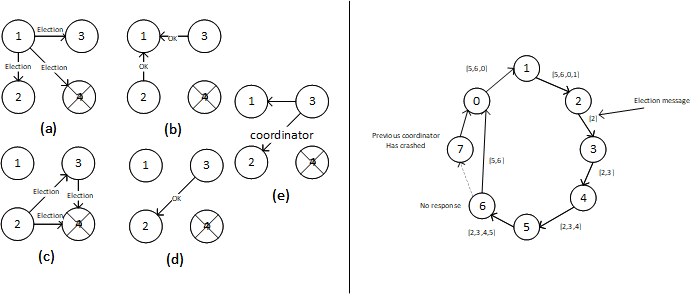
\includegraphics[width=1\linewidth]{leaderElection/data}
	\caption{The bully election on the right and to the left A ring algorithm}
	\label{fig:data}
\end{figure}
As seen in figure \ref{fig:data} on the left. The bully election algorithm starts by (a) Process 1 holds an election because it notices 4 has crashed. (b)
Processes 2 and 3 respond, telling 1 to stop. (c) Now 2 and 3 each hold an
election. (d) Process 3 tells 2 to stop. (e) Process 3 wins and tells everyone.

As seen in figure \ref{fig:data} on the right. The ring algorithm and it beings by 2 and 5 start election message independently. Both messages continue to circulate the ring and at some point both messages will go all the way around. In the last step not shown on the figure 2 and 5 convert their election messages to coordinator message and then all processes recognize highest numbered process as new coordinator.